%to have line numbers
%\RequirePackage{lineno}
\documentclass[10pt, letterpaper]{article}      
\usepackage[margin=.1cm,font=small,labelfont=bf]{caption}[2007/03/09]
%\usepackage{endnotes}
%\let\footnote=\endnote
\usepackage{setspace}
\usepackage{longtable}                        
\usepackage{anysize}                          
\usepackage{natbib}                           
%\bibpunct{(}{)}{,}{a}{,}{,}                   
\bibpunct{(}{)}{,}{a}{}{,}                   
\usepackage{amsmath}
\usepackage[% draft,
pdftex]{graphicx} %draft is a way to exclude figures                
\usepackage{epstopdf}
\usepackage{hyperref}                             % For creating hyperlinks in cross references
\hypersetup{pdfborder={0 0 0.4}} %have nice light boxes on refs

% \usepackage[margins]{trackchanges}

% \note[editor]{The note}
% \annote[editor]{Text to annotate}{The note}
%    \add[editor]{Text to add}
% \remove[editor]{Text to remove}
% \change[editor]{Text to remove}{Text to add}

%TODO make it more standard before submission: \marginsize{2cm}{2cm}{1cm}{1cm}
\marginsize{1cm}{1cm}{.5cm}{.5cm}%{left}{right}{top}{bottom}   
					          % Helps LaTeX put figures where YOU want
 \renewcommand{\topfraction}{1}	                  % 90% of page top can be a float
 \renewcommand{\bottomfraction}{1}	          % 90% of page bottom can be a float
 \renewcommand{\textfraction}{0.0}	          % only 10% of page must to be text

 \usepackage{float}                               %latex will not complain to include float after float

\usepackage[table]{xcolor}                        %for table shading
\definecolor{gray90}{gray}{0.90}
\definecolor{orange}{RGB}{255,128,0}

\renewcommand\arraystretch{.9}                    %for spacing of arrays like tabular

%-------------------- my commands -----------------------------------------
\newenvironment{ig}[1]{
\begin{center}
 %\includegraphics[height=5.0in]{#1} 
 \includegraphics[height=3.3in]{#1} 
\end{center}}

 \newcommand{\cc}[1]{
\hspace{-.13in}$\bullet$\marginpar{\begin{spacing}{.6}\begin{footnotesize}\color{blue}{#1}\end{footnotesize}\end{spacing}}
\hspace{-.13in} }

%-------------------- END my commands -----------------------------------------



%-------------------- extra options -----------------------------------------

%%%%%%%%%%%%%
% footnotes %
%%%%%%%%%%%%%

%\long\def\symbolfootnote[#1]#2{\begingroup% %these can be used to make footnote  nonnumeric asterick, dagger etc
%\def\thefootnote{\fnsymbol{footnote}}\footnote[#1]{#2}\endgroup}	%see: http://help-csli.stanford.edu/tex/latex-footnotes.shtml

%%%%%%%%%%%
% spacing %
%%%%%%%%%%%

% \abovecaptionskip: space above caption
% \belowcaptionskip: space below caption
%\oddsidemargin 0cm
%\evensidemargin 0cm

%%%%%%%%%
% style %
%%%%%%%%%

%\pagestyle{myheadings}         % Option to put page headers
                               % Needed \documentclass[a4paper,twoside]{article}
%\markboth{{\small\it Politics and Life Satisfaction }}
%{{\small\it Adam Okulicz-Kozaryn} }

%\headsep 1.5cm
% \pagestyle{empty}			% no page numbers
% \parindent  15.mm			% indent paragraph by this much
% \parskip     2.mm			% space between paragraphs
% \mathindent 20.mm			% indent math equations by this much

%%%%%%%%%%%%%%%%%%
% extra packages %
%%%%%%%%%%%%%%%%%%

\usepackage{datetime}


\usepackage[latin1]{inputenc}
\usepackage{tikz}
\usetikzlibrary{shapes,arrows,backgrounds}


%\usepackage{color}					% For creating coloured text and background
%\usepackage{float}
\usepackage{subfig}                                     % for combined figures

\renewcommand{\ss}[1]{{\colorbox{blue}{\bf \color{white}{#1}}}}
\newcommand{\ee}[1]{\endnote{\vspace{-.10in}\begin{spacing}{1.0}{\normalsize #1}\end{spacing}\vspace{.20in}}}
\newcommand{\emd}[1]{\ExecuteMetaData[/tmp/tex]{#1}} % grab numbers  from stata

%TODO before submitting comment this out to get 'regular fornt'
\usepackage{sectsty}
\allsectionsfont{\normalfont\sffamily}
\usepackage{sectsty}
\allsectionsfont{\normalfont\sffamily}
\renewcommand\familydefault{\sfdefault}

%\usepackage[margins]{trackchanges}
\usepackage{rotating}
\usepackage{catchfilebetweentags}

\usepackage{abstract}
\renewcommand{\abstractname}{}    % clear the title
\renewcommand{\absnamepos}{empty} % originally center
%-------------------- END extra options -----------------------------------------
\date{{}\today \hspace{.2in}\xxivtime}
\title{  % remember to have Vistula University!!
  The Impact of Covid19\\ on\\ the Urban-Rural Happiness Gradient
}
\author{
Adam Okulicz-Kozaryn\thanks{EMAIL: adam.okulicz.kozaryn@gmail.com
  % \hfill I thank XXX.  All mistakes are mine.
} \\
{\small Rutgers - Camden  % and Vistula University
}\\
Rubia R. Valente\\
{\small CUNY/Baruch}
}

\begin{document}

%%\setpagewiselinenumbers
%\modulolinenumbers[1]
%\linenumbers

\bibliographystyle{/home/aok/papers/root/tex/ecta}
\maketitle
\vspace{-.4in}
\begin{center}

\end{center}


\begin{abstract}
  \noindent People in the developed world tend to be less happy in cities than
  in rural areas, i.e., ``urban-rural happiness gradient." The recent covid19
  pandemic offers an opportunity to explore one of the disadvantages of large
  cities and dense settlements: the greater spread of infectious diseases % compared to rural areas
  . Thus, in this paper, we examine how covid19 affected happiness in the largest cities compared to smaller areas using the World Values Survey. What's remarkable is a large differential or effect size pre-post pandemic for cities v smaller areas.  Cities  became 2 times less happy post-pandemic v pre-pandemic compared to smaller areas. There has been 2x decrease for United Kingdom and the Netherlands.  For Uruguay there has been an increase in
 life satisfaction across both cities and smaller places, but the increase has been 2x smaller for cities v smaller areas. % In relative terms, effect size differentials are remarkable---it is rare to see in SWB research 2x or 200\% differentials.
 In absolute terms, % effect sizes are large, too.
 while .2-.5 difference on 1-10 SWB scale is small, one must take into account the massive scale of
 urbanization: .2-.5  on 1-10 SWB scale for millions of people is a massive slump in human wellbeing. Findings are correlational, not causal. 
\end{abstract}
\vspace{.15in} 
\noindent{\sc urban, rural, urban-rural happiness gradient, happiness, life satisfaction,
  subjective wellbeing, covid19
}
\vspace{.25in} 

\begin{spacing}{1.4} %TODO MAYBE before submission can make it like 2.0
\rowcolors{1}{white}{gray90}

%  instead \ExecuteMetaData[../out/tex]{ginipov} do \emd{ginipov}

% \begin{figure}[H]
%  \includegraphics[height=3in]{../out/gov_res_trust.pdf}\centering\label{gov_res_trust}
% \caption{woo}
% \end{figure}


%TODO !!!! have input here aok_var_des



% %table centered on decimal points:)
% \begin{table}[H]\centering\footnotesize
% \caption{\label{freq_im_god} importance of God}
% \begin{tabular} {@{} lrrrr @{}}   \hline 
% Item& Number & Per cent   \\ \hline
% 1(not at all)&    9,285&  9\\
% 2&    3,555&        3\\
% 3&    3,937&        4\\
% 4&    2,888&        3\\
% 5&    7,519&        7\\
% 6&    5,175&        5\\
% 7&    6,050&        6\\
% 8&    8,067&        8\\
% 9&    8,463&        8\\
% 10&   52,385&       49\\
% Total&  107,324&      100\\ \hline
% \end{tabular}\end{table}


% % Define block styles
% \tikzstyle{block} = [rectangle, draw, fill=black!20, 
%     text width=10em, text centered, rounded corners, minimum height=4em]
% \tikzstyle{b} = [rectangle, draw,  
%     text width=6em, text centered, rounded corners, minimum height=4em]
% \tikzstyle{line} = [draw, -latex']
% \tikzstyle{cloud} = [draw, ellipse,fill=black!20, node distance = 5cm,
%     minimum height=2em]
    
% \begin{tikzpicture}[node distance = 2cm, auto]
%     % Place nodes
%     \node [block] (lib) {liberalism, egalitarianism, welfare};
%     \node [block, below of=lib] (con) {conservatism, competition, individualism};
%     \node [cloud, right of=con] (ls) {well-being};
%     \node [block, below of=ls] (cul) {genes, culture};
%     \node [b, left of =lib, node distance = 4cm] (c) {country-level};
%     \node [b, left of =con,  node distance = 4cm] (c) {person-level};
%     % Draw edges
%     \path [line] (lib) -- (ls);
%     \path [line] (con) -- (ls);
%     \path [line,dashed] (cul) -- (ls);
% \end{tikzpicture}


%PUT THIS NOTE, polish and put to /root/author_what_data --ALWAYS
%stick here stuff as i run it!!! maybe comment out later...

'Here is the great city: here have you nothing to seek and everything to lose.' Nietzsche\\

\section{Introduction} 


Covid19 has changed our way of life \citep{olasov22}. Many changes are persistent so far
   and there seems to be no coming back. One of the key areas
  changed is urbanism. Pre-pandemic there has been city renewal, rebirth, and indeed
  triumphalism. Post-pandemic there is urban scepticism, scare, and indeed, in
  some cases, collapse. 
 %
Timing is everything. Ed Glaeser wrote a bestselling book 'Triumph of the city'
\citep{peck16} just several years before the collapse of the city. Many cities are hollowed out in important ways by the covid19 pandemic.

% Celebrity urbanlogy \citep{peck16} does not take into account inherently urban
% disadvantages such as higher crime or infectious disease spread. What is missed
% is that crime disease are urban feature--they are higher per capita in cities
% because city itself increases them. These are universal laws, like physics laws,
% and they are best illustrated with a graph

The covid19 pandemic % changed our way of life and highlighted the vulnerability and disparities of society at large. In particular, it
 has exposed the differences between urban and rural % areas
. % The impact of covid19 varied significantly depending on where people lived--
 A person's chance of getting the virus and surviving it was closely associated to their zipcode \citep{chen2021}. Urban areas were the epicenters of the virus outbreak: the dense population and inevitable close proximity to others, a defining feature of cities, resulted in rapid transmission and a fertile ground for infection. % Indeed, studies have long documented that
 One of the disadvantages of city life is the increased spread of infectious
 disease\footnote{See for example, ``SIR Models for Spread of Disease'' \citep{newman2002spread,cooper2020sir}. } \citep{bettencourt10,bettencourt07}. %Indeed, it could be called ``law'', like physics laws such as gravity.
The transmission of infectious disease is a social contact process. To be sure,
although the scale of covid19 was unparalleled, all major infectious disease
outbreaks in the past, e.g., SARS, Ebola, Flu, occurred in metropolitan
areas.{\color{red}rubia: cite}  Rural areas in contrast, given their lower population density and geographic isolation, provide a natural social distancing environment that slows the spread of infectious viruses. As such, covid19 affected cities more than smaller areas \citep{stier2021early}.


%We know that one of the disadvantages of city is increased infectious disease spread% Indeed such population scaling is so consistent and
% strong, it is universal
%\citep{bettencourt10,bettencourt10b,bettencourt07}. %Indeed, it could be called ``law'', like physics laws such as gravity.
%Disease transmission is a social contact process. %https://player.slideplayer.com/16/4964980/# slide14 i guess he meant sth like these:
%https://www.maa.org/press/periodicals/loci/joma/the-sir-model-for-spread-of-disease-the-differential-equation-model
%https://sites.me.ucsb.edu/~moehlis/APC514/tutorials/tutorial_seasonal/node2.html


% Massive infectious diseases happene every now and then, SARS, Ebola, etc, and recently COVID19. The
% research hypothesis is that as cities suffer disporportionately from infectious
% diseases, city happiness decreased disproportionaly as well with covid19.


   %
%  In present study we take a human development perspective using a measure of
%  human flourishinng, subjective wellbeing (swb).
%  Boilerplate from sen stiglitz and UN!! (see slides from cSWB).

In the present study, we take a development perspective using a measure of human
development, progress, or flourishing, subjective wellbeing (SWB). Our 
 hypothesis is that since cities suffer disproportionately from
infectious diseases, city happiness decreased disproportionately during the
covid19 pandemic.

We start with a brief overview of how covid19 impacted
different aspects of life in urban versus rural areas. Next we present the
underlying theory, the urban-rural happiness gradient theory suggesting that
happiness should be observed in the least dense and heterogeneous places, such
as rural areas. We end the literature review by pointing to gaps in the
literature and pro-urban proclivity pre-pandemic. Our empirical analysis follows
and we conclude with a discussion of results and future research. %takeaways for policy and practice.



\section{Urban-Rural Happiness Gradient}


\citet{aokcities} investigated global differences in satisfaction with urban
life. In developed countries, rural residence increased happiness at double the
rate that big-city residence boosted malaise, a pattern most pronounced in
societies with an Anglo-Saxon heritage.  \citet{easterlin10al} found that in
more advanced developed countries, rural areas approach or exceed urban areas in
life satisfaction, while in developing countries the low levels of economic
development result in gaps favoring urban areas over rural areas when it comes
to income, education and life satisfaction. Over last decade many studies have 
explored the urban-rural happiness gradient around the world. This body of
research has indicated that generally, rural residents tend to report higher
levels of happiness compared to their urban counterparts--for recent review see
\citet{aok21}. There are notable exceptions, however, Millenials in the US for example \citep{aok-swbGenYcity18}.
 
In a recent paper, \citet{easterlin23} points out that only few
studies examine the effect of covid19 on SWB.  \citet{easterlin23} does an
overal analysis for Europe, but misses urban-rural differential. Thus, this is
the first study on the topic.


Health is one of the strongest predictors of SWB, if not the very
strongest--decent health is clearly necessary for SWB \citep[e.g.,][]{campbell76etal}--health is expected to be
strongly linked with SWB. And cities suffer disproportionately during pandemics
in terms of health.  
 %
 Again, cities are hotbeds of infectious disease--infections are promoted by
proximity and close contact between humans--by definition cities offer the
most fertile ground for infectious disease spread.

There are detailed data for the geography of pandemic in the  US, and other
countries likely followed a similar pattern-- 
%
It is especially large central metropolitan areas that are mostly affected as
  compared to fringe metros and medium cities \citep{curtin2022covid}.
  %https://www.cdc.gov/nchs/products/databriefs/db447.htm
  %
 The urban covid19 disadvantage was at the beginning of the pandemic with
 incidence almost 2x and mortality almost 3x in urban v rural areas. Then rates
 converge, and towards the end of the pandemic cities recover and rural areas
 have higher rates \citep{cuadros2021dynamics}. 
%https://www.ncbi.nlm.nih.gov/pmc/articles/PMC8061094 %(tab1)
%https://www.ers.usda.gov/data-products/chart-gallery/gallery/chart-detail/?chartId=100740
 Still, the urban (not rural) scare remains--cities are hit first, and proximity
 to others and chance of infection is astronomically greater in the cities. 
 %
%  The graph illustates the trajectory well:
% https://www.cdc.gov/mmwr/volumes/69/wr/mm6946a6.htm
 It needs to be remembered the infection rates are reported per capita, say per 100,000 population. If it was per
area, say sq km, i.e., how much disease there is in an area, the urban disadvantage
would have been astronomical. For instance in NYC population density is about
11k/sq km, whereas in Montana it is about 3/sq km, about 3600x difference.



\section{Data}

We use the World Values Survey 7-wave 1981-2022 cumulative file freely available
at \url{worldvaluessurvey.org}. We
proceed as follows with the sample selection: the rate of covid19 infection
increased substantially later in 2020, peaked in 2021, and still had a
considerable effect in 2022. Hence, we restrict the covid19 period sample to
2021 and 2022 (2023 is not available yet). Data in
2021 are only available for small developing countries with small
cities (not much urbanism): Armenia, Kenya, Maldives, Morocco, and
Venezuela.\footnote{Kenya does have large cities but it has been
  largery spared from covid19--at 50m population it only had 342k cases (less
  than 1\%) and 6k deaths \url{https://coronavirus.jhu.edu/region/kenya}.  
  Likewise, there are large cities in Venezuela, but it is a dictatorship
  largely cut off from the world, which might have protected it from
  covid19--despte being about 30m there were only .5m cases and 5k deaths, while
  in neighboring Colombia of 50m there were 6.3m cases and 142k deaths
  \url{https://coronavirus.jhu.edu/region/venezuela}} Hence, for 2022 we obtain:
Czechia, Libya, Netherlands, Northern Ireland, Slovakia, United Kingdom, and Uruguay. Next, we checked sample sizes by year and urbanicity (X049) for each country. We
excluded: Czechia--it had no city with a population larger than 500k before
2022; Libya--there were only 7 respondents in cities larger than 500k before
2022; Northern Ireland--the total sample size is 447 and there's data only for
one wave; Slovakia--only 61 respondents in cities with a population larger than
500k pre-2022. Which leaves us with United Kingdom (GBR), the Netherlands (NLD), and
Uruguay (URY).


\section{Results}

The results are set in figure \ref{barA}. Each panel shows results for a
separate country: United Kingdom (GBR), the Netherlands (NLD), and Uruguay
(URY). Y axis is life satisfaction. X-axis is urban-rural gradient--degrees of
urbanicity or urbanness. Blue bars show pre-pandemic averages (year varies by country), and green bars show pandemic/post-pandemic averages (2022). 

\begin{figure}[H]
 \includegraphics[width=7in]{barA.pdf}\centering
\caption{\label{barA}Life satisfaction ($1=unhappy$ to $10=happy$) means with 95\% CI against rural urban gradient categories. $GBR=$ United Kingdom, $NLD=$ Netherlands, $URY=$ Uruguay.}
 \end{figure}

In both, United Kingdom (GBR) and the Netherlands (NLD) the biggest difference
pre-post pandemic (blue v green bar) is for the largest places ($>.5m$). Uruguay
(URY), on the other hand, experienced an increase in SWB across urbanicity, but
the largest places ($>.5m$) increased least. Thus, across the three countries,
we find support for our hypothesis of large cities happiness suffering
disporportionately post pandemic. 
Next, we repeat the above figure \ref{barA}, but with more detailed urban-rural
classification to explore nuances in figure \ref{bar2}.

\begin{figure}[H]
 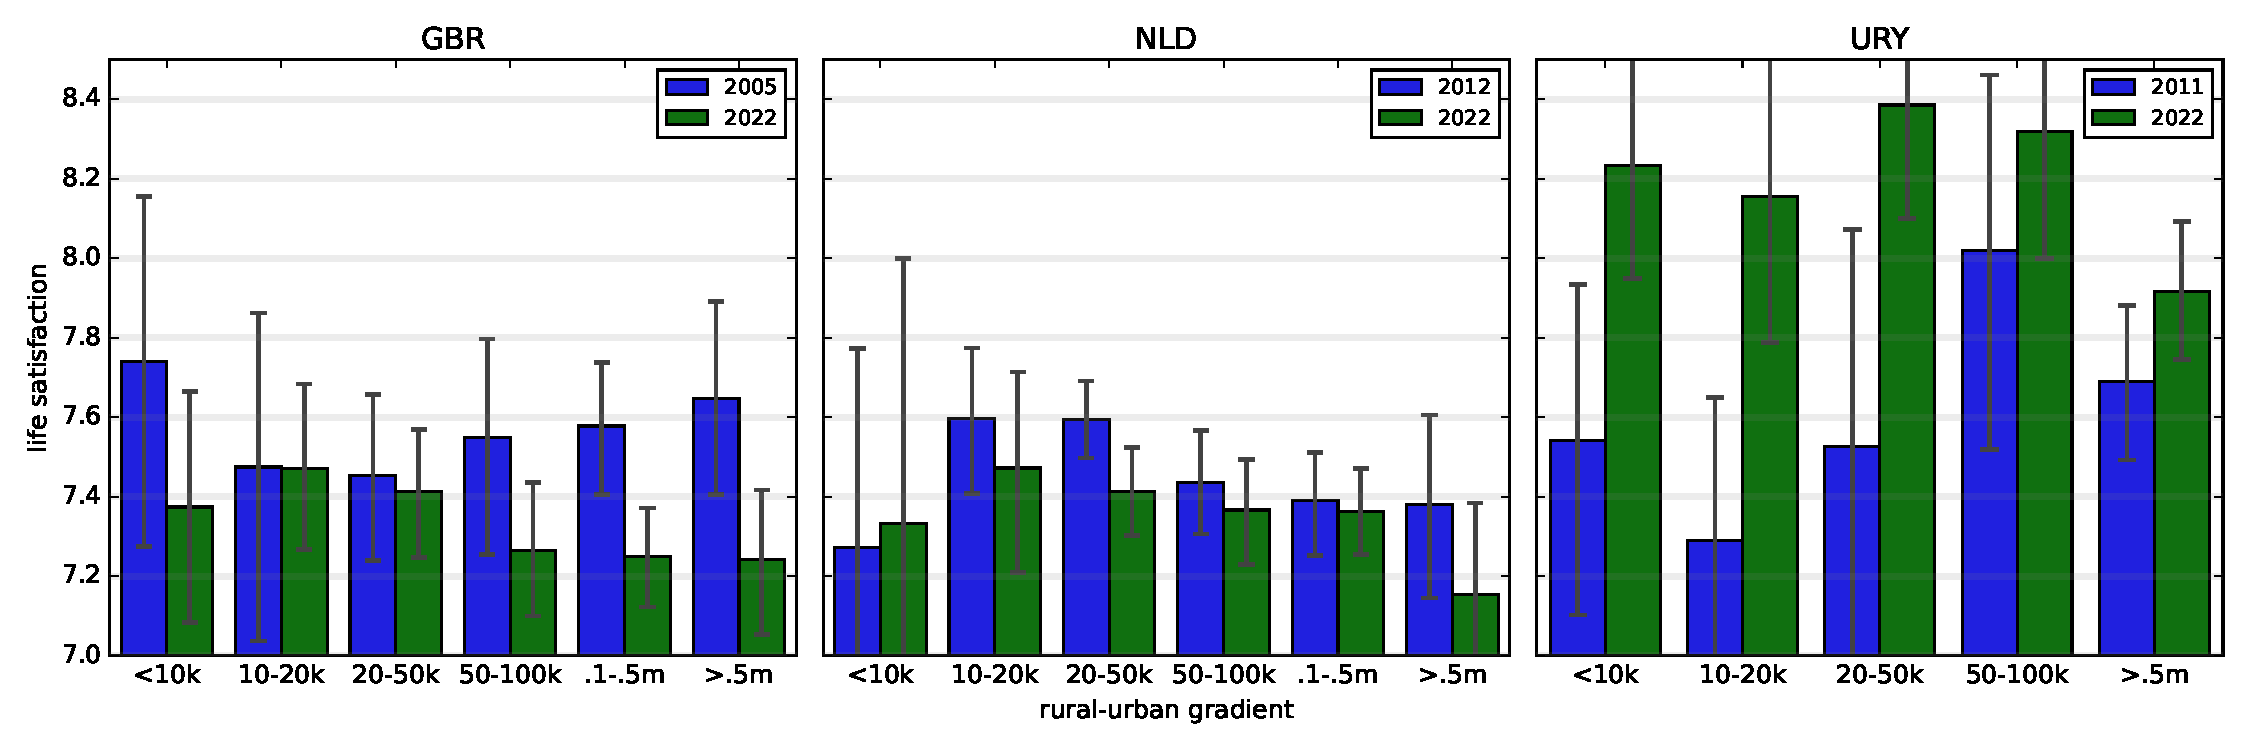
\includegraphics[width=7in]{bar.pdf}\centering
\caption{\label{bar2}Life satisfaction ($1=unhappy$ to $10=happy$) means with 95\% CI against rural urban gradient categories. $GBR=$ United Kingdom, $NLD=$ Netherlands, $URY=$ Uruguay. Note: URY is missing .1-.5m cat due to small cell sizes.}
 \end{figure}

In United Kingdom, pre-pandemic, the happiest places were the smallest ($<-10k$), while during the pandemic, both the smallest and largest places were most affected and saw significant reduction in SWB. It is unexpected to see this reduction in the smallest places, and the result could be due to some country specific factors.

In the Netherlands, there's not much change in subjective well being in smaller
places pre and post the pandemic, except for the largest cities where there's a
significant drop in SWB as expected. There was also a smaller drop in 10-20, and
especially 20-50 categories. 

Uruguay, a developing country, shows a different story: SWB increased across urbanicity, including the largest areas ($>$500k), but that's also where the smallest increase occurred, as expected.
Many of the CI are wide, and it is not clear which differences are significant.  
%TODO fix Figure 1, so that the CI are shown completely, it's cut off for Uruguay. meh no jaja


Next, we test the differences with regression. First, since the focus is on cities v smaller areas (rural and towns), for simplicity, we collapsed categories up to .5m into one as rural and towns, and contrast this category with cities (larger than .5m). 

There are also two technical reasons for this approach. It is a simpler exposition to have urban dichotomy as opposed to a full gradient, given that we also have two other
breakdowns: pre-post COVID and by country. And, critically, the cell sizes run small with too many breakdowns for this relatively small dataset. When more data becomes available, future research should test the full urban-rural gradient.  

Our hypothesis is that while the pandemic decreased SWB in general, we expect to see an even greater SWB decrease in cities. We are focused on the pre-post pandemic differences in SWB levels in big city versus smaller areas. 

Bivariate regression results are set in table \ref{a}.
We first separate our analyses by country and then within each country by rural and
towns ($<.5m)$ v cities $(>.5m)$. We regress life satisfaction on a year dummy
for 2022 with the base case being the latest pre-pandemic wave as shown in
figures \ref{barA} and \ref{bar2}. 
% First we could look at overall change in happiness pre-post pandemic or such % change for all areas except large cities.



\begin{spacing}{.9} \begin{table}[H]\centering   \begin{scriptsize} \begin{tabular}{p{1.8in}p{.5in}p{.5in}|p{.5in}p{.5in}|p{.5in}p{.5in}|p{.5in}p{.5in}p{.5in}p{.5 in}p{.5in}p{.5 in}}\hline&\multicolumn{2}{c}{GBR}&\multicolumn{2}{c}{NLD}&\multicolumn{2}{c}{URY}\\                     &   $<.5m$   &     $>.5m$   &   $<.5m$   &     $>.5m$   &   URYrurTow   &     URYcity   \\
2022                &       -0.21** &       -0.41** &       -0.12** &       -0.23   &        0.75***&        0.23+  \\
constant            &        7.54***&        7.65***&        7.50***&        7.38***&        7.54***&        7.69***\\
N                   &        3111   &         521   &        3572   &         373   &        1154   &         836   \\
 \hline + 0.10 * 0.05 ** 0.01 *** 0.001; robust std err \end{tabular}\end{scriptsize}\caption{\label{a}OLS regressions of life satisfaction.}\end{table} \end{spacing}

 Effect sizes on the year 2022 dummy are the bar length differences from fig \ref{barA}. For GBR the difference pre-post pandemic is about .2 for rural areas and towns ($<.5m$), and the difference for cities $(>.5m)$ is about .4, and so forth for NLD and URY.
 %
 A remarkable finding in our analysis is the roughly 2 times difference for GBR and NLD, and 3 times difference for URY--this is a strong differential. When comparing cities $(>.5m)$ versus smaller areas ($<.5m$), cities became 2 to 3 times less happy post-pandemic compared to pre-pandemic levels.
 
Still one of the coefficients for NLD is not significant, and only weakly
significant for URY, and there is left out variable bias. {Differences in SWB levels should be even bigger when controlling for SWB predictors as the urban rural happiness gradient often emerges only after controlling for SWB predictors \citep{aok21}.} Hence, we elaborate our models with SWB predictors in table \ref{b}.


\begin{spacing}{.9} \begin{table}[H]\centering   \begin{scriptsize} \begin{tabular}{p{1.8in}p{.5in}p{.5in}|p{.5in}p{.5in}|p{.5in}p{.5in}|p{.5in}p{.5in}p{.5in}p{.5 in}p{.5in}p{.5 in}}\hline\hline&\multicolumn{2}{c}{GBR}&\multicolumn{2}{c}{NLD}&\multicolumn{2}{c}{URY}\\                     &   $<.5m$   &     $>.5m$   &   $<.5m$   &     $>.5m$   &   URYrurTow   &     URYcity   \\
2022                &       -0.18*  &       -0.39+  &       -0.20***&       -0.45** &        0.42***&        0.21   \\
income              &        0.09***&        0.01   &        0.06***&        0.14***&        0.07*  &        0.13***\\
age                 &       -0.03*  &       -0.08** &       -0.02+  &       -0.06+  &        0.00   &       -0.06** \\
age2                &        0.00** &        0.00** &        0.00** &        0.00*  &       -0.00   &        0.00** \\
male                &       -0.18** &       -0.13   &       -0.11*  &       -0.27+  &        0.06   &        0.19   \\
married or living together as married&        0.53***&        0.74***&        0.44***&        0.23   &        0.46** &        0.06   \\
divorced/separated/widowed&        0.07   &        0.15   &       -0.11   &       -0.14   &       -0.37+  &       -0.19   \\
autonomy            &       -0.11*  &       -0.07   &       -0.11** &       -0.01   &       -0.06   &        0.06   \\
freedom             &        0.44***&        0.42***&        0.35***&        0.43***&        0.43***&        0.36***\\
trust               &        0.12+  &        0.42** &        0.43***&        0.28+  &       -0.05   &        0.10   \\
postmaterialist     &       -0.05   &       -0.18   &       -0.11*  &        0.14   &       -0.02   &        0.15   \\
god important       &        0.01   &        0.05*  &        0.02*  &       -0.01   &        0.05** &        0.06** \\
constant            &        4.08***&        5.95***&        4.59***&        4.80***&        3.47***&        4.58***\\
N                   &        1985   &         309   &        2283   &         237   &         736   &         579   \\
 \hline + 0.10 * 0.05 ** 0.01 *** 0.001; robust std err \end{tabular}\end{scriptsize}\caption{\label{b}OLS regressions of life satisfaction.}\end{table} \end{spacing}

The elaborated models in table \ref{b} confirm our earlier results. We find that there's again roughly a 2 times difference for GBR and NLD, while for URY the differential is reduced from about 3 times to roughly 2 times as well. 

As a robustness check we add ``health'' as a control variable in table \ref{c}. It is important to underscore that there's a confounding effect between pre-post covid19 and health by definition. And there will also be confounding effects between urbanicity and health since covid19 is more prevalent in cities as previously discussed.  Hence, these regressions are less useful in determining pre-post covid19 urban-rural differentials. Taking into account health, the results on the over-time SWB difference are smaller and less significant, as expected.
Remarkably though, we find that the urbanicity differentials even
though less statistically significant, are still about 2 times larger for GBR
and URY and even stronger for NLD. Arguably the high infections rate of covid19
in cities is in addition to other urban problems such as misanthrophy and
overall malaise \citep{aok22,wilson85,rosenberg56,aok-swbGenYcity18,fischer73,fischer76}. Future research is needed. 

\begin{spacing}{.9} \begin{table}[H]\centering   \begin{scriptsize} \begin{tabular}{p{1.8in}p{.5in}p{.5in}|p{.5in}p{.5in}|p{.5in}p{.5in}|p{.5in}p{.5in}p{.5in}p{.5 in}p{.5in}p{.5 in}}\hline\hline&\multicolumn{2}{c}{GBR}&\multicolumn{2}{c}{NLD}&\multicolumn{2}{c}{URY}\\                     &   $<.5m$   &     $>.5m$   &   $<.5m$   &     $>.5m$   &   URYrurTow   &     URYcity   \\
2022                &       -0.12   &       -0.26   &       -0.06   &       -0.24+  &        0.44***&        0.23   \\
health              &        0.48***&        0.67***&        0.62***&        0.77***&        0.56***&        0.32** \\
income              &        0.05** &       -0.01   &        0.04***&        0.08** &        0.05   &        0.12***\\
age                 &       -0.02*  &       -0.07*  &       -0.01   &       -0.03   &        0.01   &       -0.05*  \\
age2                &        0.00** &        0.00** &        0.00** &        0.00+  &       -0.00   &        0.00*  \\
male                &       -0.16*  &       -0.15   &       -0.09+  &       -0.23+  &       -0.01   &        0.14   \\
married or living together as married&        0.49***&        0.60** &        0.38***&        0.21   &        0.41** &        0.04   \\
divorced/separated/widowed&        0.05   &        0.20   &       -0.15   &       -0.27   &       -0.36+  &       -0.16   \\
autonomy            &       -0.12** &       -0.09   &       -0.10** &        0.07   &       -0.09   &        0.04   \\
freedom             &        0.38***&        0.29***&        0.29***&        0.31***&        0.40***&        0.35***\\
trust               &        0.07   &        0.28*  &        0.34***&        0.21   &       -0.07   &        0.01   \\
postmaterialist     &       -0.05   &       -0.26+  &       -0.09*  &        0.06   &        0.01   &        0.12   \\
god important       &        0.01   &        0.02   &        0.02+  &        0.00   &        0.05** &        0.06** \\
constant            &        2.72***&        4.29***&        2.46***&        2.01*  &        1.31+  &        3.31***\\
N                   &        1985   &         309   &        2279   &         236   &         736   &         578   \\
 \hline + 0.10 * 0.05 ** 0.01 *** 0.001; robust std err \end{tabular}\end{scriptsize}\caption{\label{c}OLS regressions of life satisfaction.}\end{table} \end{spacing}



Finally, we pool data for the three countries together--
%Our final set of results shows all pooled data together. Earlier we split the sample by pre-post COVID, and large city versus town and rural areas for simplicity and ease of interpretation. However, 
it is useful to formally test the differences with interactions in table \ref{d}.




\begin{spacing}{.9} \begin{table}[H]\centering   \begin{scriptsize} \begin{tabular}{p{1.8in}p{.5in}p{.5in}p{.5in}p{.5in}p{.5in}p{.5in}p{.5in}p{.5in}p{.5in}p{.5 in}p{.5in}p{.5 in}}\hline                     &          a1   &          a2   &          a3   &          a4   &          a5   \\
post pandemic            &       -0.20** &       -0.13+  &       -0.10   &       -0.02   &       -0.18*  \\
city lg500k&        0.05   &        0.19*  &        0.20*  &        0.11   &        0.07   \\
post pandemic $\times$ city lg500k&       -0.26*  &       -0.26*  &       -0.26*  &       -0.21+  &       -0.15   \\
United Kingdom      &       -0.04   &        0.03   &        0.08   &       -0.01   &       -0.04   \\
Uruguay             &        0.82***&        0.92***&        0.95***&        0.68***&        0.43***\\
2011                &       -0.82***&       -0.72***&       -0.54***&       -0.47***&       -0.44***\\
2012                &       -0.10   &        0.15+  &        0.11   &        0.02   &        0.05   \\
income              &               &        0.14***&        0.13***&        0.08***&        0.08***\\
age                 &               &       -0.05***&       -0.04***&       -0.03***&       -0.03***\\
age2                &               &        0.00***&        0.00***&        0.00***&        0.00***\\
male                &               &       -0.16***&       -0.17***&       -0.16***&       -0.11** \\
married or living together as married&               &        0.46***&        0.46***&        0.39***&        0.44***\\
divorced/separated/widowed&               &        0.01   &        0.01   &       -0.03   &       -0.07   \\
god important       &               &               &        0.03***&        0.03***&        0.02***\\
trust               &               &               &        0.38***&        0.25***&        0.26***\\
postmaterialist     &               &               &       -0.04   &       -0.05+  &       -0.04   \\
autonomy            &               &               &       -0.10***&       -0.10***&       -0.09***\\
health              &               &               &               &        0.71***&               \\
freedom             &               &               &               &               &        0.40***\\
constant            &        7.58***&        7.42***&        7.14***&        4.40***&        4.47***\\
N                   &        9196   &        7746   &        6038   &        6032   &        5970   \\
 \hline + 0.10 * 0.05 ** 0.01 *** 0.001; robust std err \end{tabular}\end{scriptsize}\caption{\label{d}OLS regressions of life satisfaction.}\end{table} \end{spacing}

 We start with a basic model where we regress life satisfaction on a dummy for the largest cities, and post-pandemic wave dummy where ``post pandemic'' $=1$ if $year=2022$. We also include country dummies, as we now pull all the data together. Finally, we also include year dummies in addition to pre-post dummy since data were collected in different countries in different years. 

In column a1, as expected we see that post pandemic SWB went down by -.2, and
especially so for cities by an additional -.26. When adding basic controls in
a2, we find that the main variable of interest testing our hypothesis, post
pandemic$*$city lt 500k, stays about the same at -.26. We include an extended
list of controls in a3, and again  the  coefficient stays at -.26. It is only
after adding ``health'' in model a4 that it the coefficient slightly drops to
-.21. Finally,  the addition of freedom in model a5 cuts the effect most
substantially to -.15 and loses statistical significance. Future research should
further explore why controlling for ``freedom'' removes the effect.\footnote{The
  original WVS code for the freedom variable is A173: "Some people feel they
  have completely free choice and control over their lives, while other people
  feel that what they do has no real effect on what happens to them. Please use
  this scale where 1 means 'none at all' and 10 means 'a great deal' to indicate
  how much freedom of choice and control you feel you have over the way your
  life turns out." A rationale to look at freedom is that it confounds with
  city; i.e., city has more freedom than rural at least in some senses. The idea
  goes back at least to Ferdinand Toennies' "Gemeinschaft und Gesellschaft" \citep{tonnies57}--city air is free--e.g., nonstandard/nonconformist types such as LGBTQ are more free in a city.}



\section{Conclusion and Discussion}

%Rural at least in the US---millennial's paper that city swb was doing better v rural arguably
%because rural has been left behind. 
The covid19 pandemic has adversely impacted SWB around the world, but especially
in large cities and metropolitan areas. Before the pandemic, city happiness was
on the rise relative to rural areas \citep{millennials}. As rural areas have
been left behind \citep{hansonCityJournalautumn15}, the rural happiness
advantage has decreased. A rural Californian explains \citep[][p. 2]{fullerNYT17monD}:

\begin{quote}``In the rural parts of the state we drive more miles, we drive older cars, our economy is an agriculture- and resource-based economy that relies on tractors. You can't move an 80,000-pound load in an electric truck. They've devastated ag jobs, timber jobs, mining jobs with their environmental regulations, so, yes, we have a harder time sustaining the economy, and therefore there's more people that are in a poorer situation.''
\end{quote}

Ironically, the covid19 pandemic made the economic advantage and prosperity of
cities quickly wither away. The pandemic created significant economic turmoil
particularly in large urban centers: as businesses and industries shut down,
millions lost their jobs, and thousands fled to the suburbs or smaller places,
hoping to avoid human interaction and protect themselves against the
virus. Places like New York City, that were vibrant and full of life, became
dull and empty. Still, as of 2024, much of commercial real estate in urban cores
is empty.

Urban and rural areas experienced and coped with the pandemic very
differently. Urban areas became the center of coronavirus outbreaks around the
world, and many cities saw their healthcare systems become quickly overwhelmed
given the magnitude of the virus--makeshift hospitals and makeshift morgues were
set up in cities like New York City.

There's always a strong correlation between subjective well being and
health. Health is the key predictor of happiness--almost no one considers health
unimportant \citep[e.g.,][]{campbell76etal}. The virus not only made people severely ill, but it prevented people who had any other health emergencies or issues from being properly taken care of (e.g., cancer, heart disease, diabetes). This was particularly an issue in large metropolitan areas. The number of people who's health was directly or indirectly affected by covid19 is significantly larger then the reported statistics of covid19 infection. 
Thus, it no surprise that our findings show such a significant and relatively
large drop in happiness levels in cities as compared to smaller places.

Understanding the discrepancies is important because policymakers can implement
policies targeted to create a more healthy and livable environment for urban and
rural residents based on the different challenges they experience to foster
happiness. The spread of infectious disease in cities is unavoidable and will
likely happen again in the near future. Learning from the challenges brought by
covid19 might result in lifesaving, health and happiness promoting measures.


Again, only initial phase of infection per capita is greater in cities, then urban rural rates converge and in last stage are higher in rural as cities got hit first and recover first. But there is arguably a strong psychological effect, urban scare, that will also last well after pandemic for the foreseeable future. Likewise, urban quality of life v rural quality of life even given the same per capita infection is very different--one can easily go about daily life and even enjoy most rural activities in rural areas, while the opposite is true in cities--city way of life during the pandemic is unbearable.

The massive difference in population density of urban v rural needs to be
highlighted. Again, NYC population density is about 11k/sq km, whereas in
Montana it is about 3/sq km, about 3600x difference. Even if infection rate were
similar across urban-rural, the difference in infection rate per sq km is
massive. And this is one key factor behind urban scare--the sheer number of
infections in one's proximity is astronomical.

Many thought that covid19 may be largely gone and cities safe to return to. One of the authors of this study was reckless enough to go to a large city, New York City, and surely enough just got infected with covid19 this summer (2023) when we were revising this paper.  
 %
President Trump has called covid19 "Chinese Virus" to pinpoint the geographic
origin, but indeed a more descriptive geographic term would be "city virus." We
advise the readers to keep away from large cities--you will be safer from
infectious disease and happier.

In many ways, cities cannot be fixed--there is inherent conflict, dysfunction
and even misanthropy in metropolis \cite{wirth38,fischer72,aok22,thrift05,amin06,aokCityBook15,peck16}. 
 %
Others would argue that a city can be fixed and made happier \citep[for a review
see][]{ballas13}. \citet{olasov22} offers many ideas by 10 philosophers. For
instance, to reimagine cities to offer convivial and sensual shared space for shared pleasure, `` a mesh of small, safe, intimate places, rather than a series of grand urban projects.''


\section{Limitations and Future Research}

As more data becomes available, it will be instructive to closely examine
countries that were most affected by covid19. Italy and the U.S., for example,
will probably show much greater negative effects on SWB than what we found in
GBR, NLD and URY. Although covid19 infection rates are significantly lower now,
and another massive pandemic could be decades ahead, we'll likely experience
covid19 lingering effects for many years to come. This could arguably include
urban scare, prevalence of misanthropolis (a metropolis full of distrust and
dislike of humankind) \citep{aok22}, and possibly an urban crisis. It would be
useful to study the long term effect on urban-rural gradient and whether covid19
has widen more permanently the urban-rural happiness gap that had been closing
\citep{aok-swbGenYcity18}.


Again, this is the first study on the topic. We are interested in
general/overall patterns to start the debate. Future research can focus on a
more direct link between inections, hospitalizations, and deaths and SWB by
linking public health data with SWB data for specific locations.


Likewise there is huge difference in infection rates across countries (e.g.,
Italy, the US, China), and across places within countries. Such differences
could be perhaps explored in a natural experiment framework where massively
infected area can be matched with a similar area but with low infection rate.


% \section*{\Huge ONLINE APPENDIX}
% \textbf{[note: this section will NOT be a part of the final version of
%   the manuscript, but will be available online instead]} %hence everything below
%                                 %is organized byu section, not subsection
% !!!
% have most of the stuff outputted to online appendix:)--start with that and then
% select stuff to paper--have brief narrative describng patterns in online app too
% !!!

% \section*{Variables' definitions, coding, and distributions}
% \label{app_var_des}


% %\input{/tmp/a.tex} %aok_var_des

% % \begin{spacing}{.9}
% %   \begin{table}[H]\centering \caption{Summary statistics.} \label{sumSta} \begin{scriptsize} \begin{tabular}{p{1.8in}p{.5in}p{.5in}p{.5in}p{.5in}p{.5in}p{.5in}p{.5in}p{.5in}p{.5in}p{.5
% %             in}p{.5in}p{.5 in}}\hline
% %         \input{/tmp/aha2.tex}
% %          \end{tabular}\end{scriptsize}\end{table}
% % \end{spacing}

% % \begin{spacing}{.9}
% %   \begin{table}[H]\centering \caption{Correlation matrix.} \label{sumSta} \begin{scriptsize} \begin{tabular}{@{}
% %           p{1.2in} rrrrrrrrrrrrr @{}}\hline
% %         \input{/tmp/ahb2.tex}\hline
% %          \end{tabular}\end{scriptsize}\end{table}
% % \end{spacing}



% Table XXX shows variable distributions. If a variable has more than
% 10 categories it is classified into bins...

% %\input .... %TODO !!!! have input here histograms

% \section*{Additional Descriptive Statistics}
% \label{app_des_sta}

% %make sure i have [H] or h! ???
% % \begin{table}[H]
% % \caption{}
% % \centering
% % \label{}
% % \begin{scriptsize}
% % \input{../out/reg_c.tex}
% % \end{scriptsize}
% % \end{table}

%\newpage
%\theendnotes
\bibliography{/home/aok/papers/root/tex/ebib.bib,covidCity.bib}

\end{spacing}
\end{document}
